\section{Solution and Results}

\subsection{Data Preparation}

The PDMS complex refractive index was constructed using a 15-oscillator Drude-Lorentz model calibrated to experimental data from Srinivasan et al. (2016). The AM1.5 solar spectrum follows ASTM G173-03 with total irradiance of 1000 W/m$^2$. Atmospheric transmittance in the 8--13 $\mu$m window was modeled based on MODTRAN mid-latitude summer conditions, with ozone absorption at 9.6 $\mu$m explicitly incorporated.

Figure \ref{fig:pdms_nk} shows the resulting PDMS complex refractive index. The extinction coefficient $k$ exhibits distinct absorption peaks corresponding to Si--O--Si asymmetric stretching (9.26 $\mu$m, $k \approx 0.08$), CH$_3$ symmetric deformation (7.94 $\mu$m, $k \approx 0.06$), and Si--C rocking vibrations (12.5 $\mu$m, $k \approx 0.12$). In the visible and near-infrared range (0.3--5 $\mu$m), PDMS is essentially transparent with $k < 10^{-5}$.

\begin{figure}[H]
  \centering
  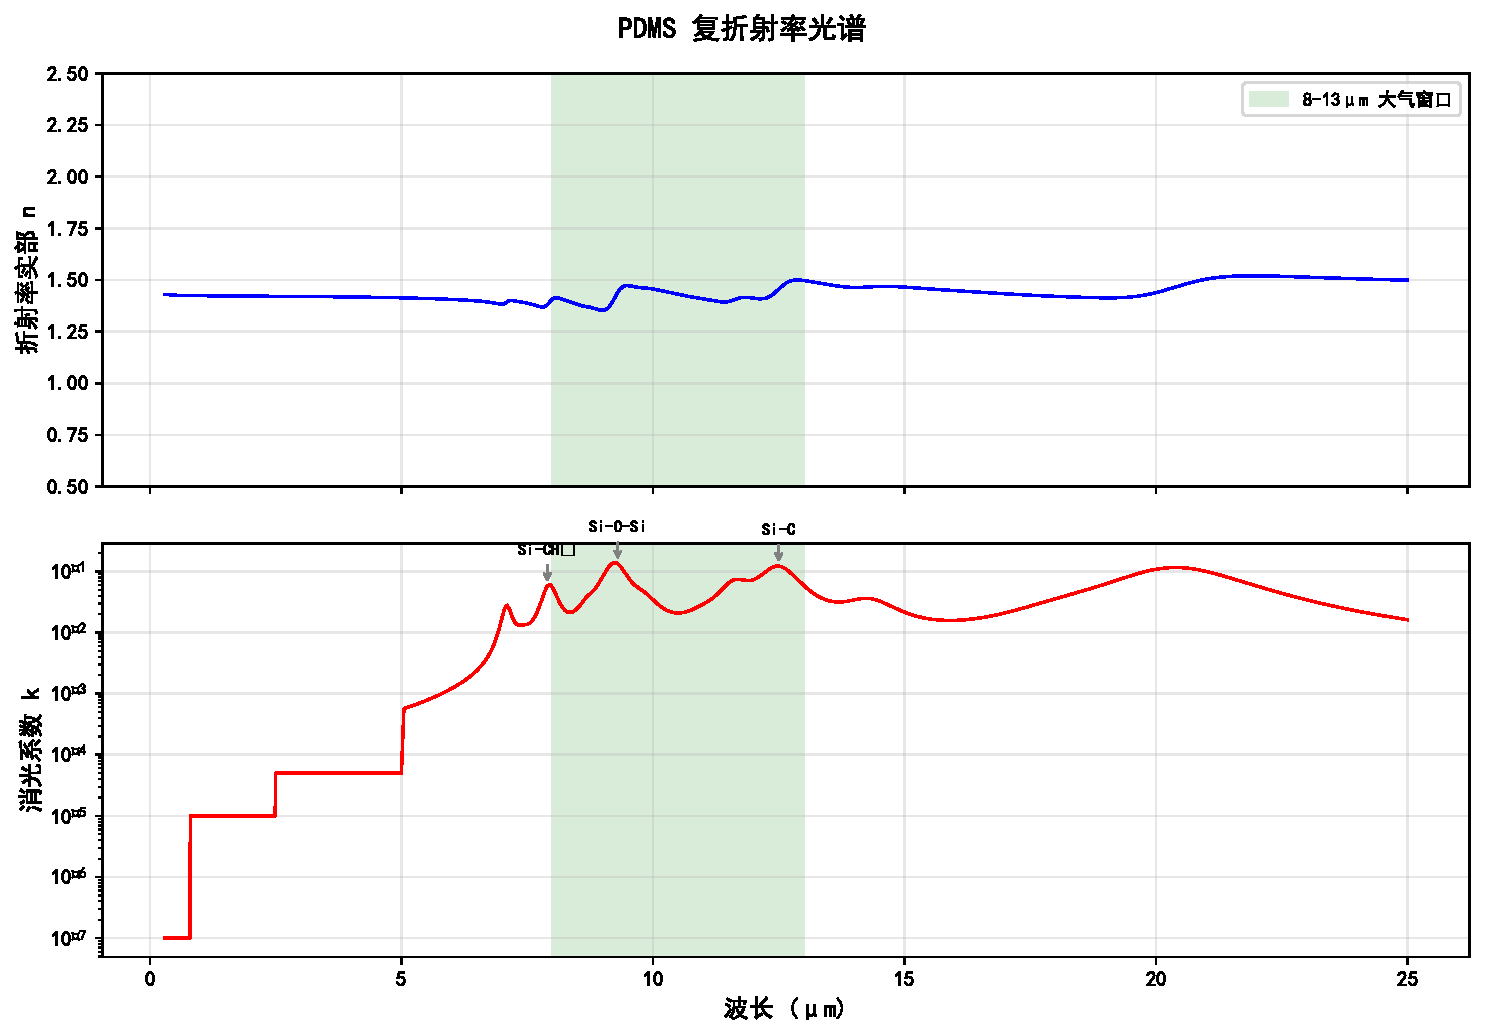
\includegraphics[width=0.90\textwidth]{../../figures/fig_pdms_refractive_index.pdf}
  \caption{PDMS complex refractive index: (top) real part $n(\lambda)$, (bottom) extinction coefficient $k(\lambda)$. The green shaded region indicates the 8--13 $\mu$m atmospheric transparency window.}
  \label{fig:pdms_nk}
\end{figure}

\subsection{Problem 1: PDMS Emissivity vs. Wavelength and Thickness}

Figure \ref{fig:emis_spectrum} presents the spectral emissivity $\varepsilon(\lambda)$ for PDMS films of varying thicknesses. For thin films ($d < 5$ $\mu$m), the emissivity spectrum exhibits pronounced interference fringes due to coherent thin-film interference. As thickness increases, these oscillations dampen and the emissivity converges toward the bulk PDMS absorption profile.

\begin{figure}[H]
  \centering
  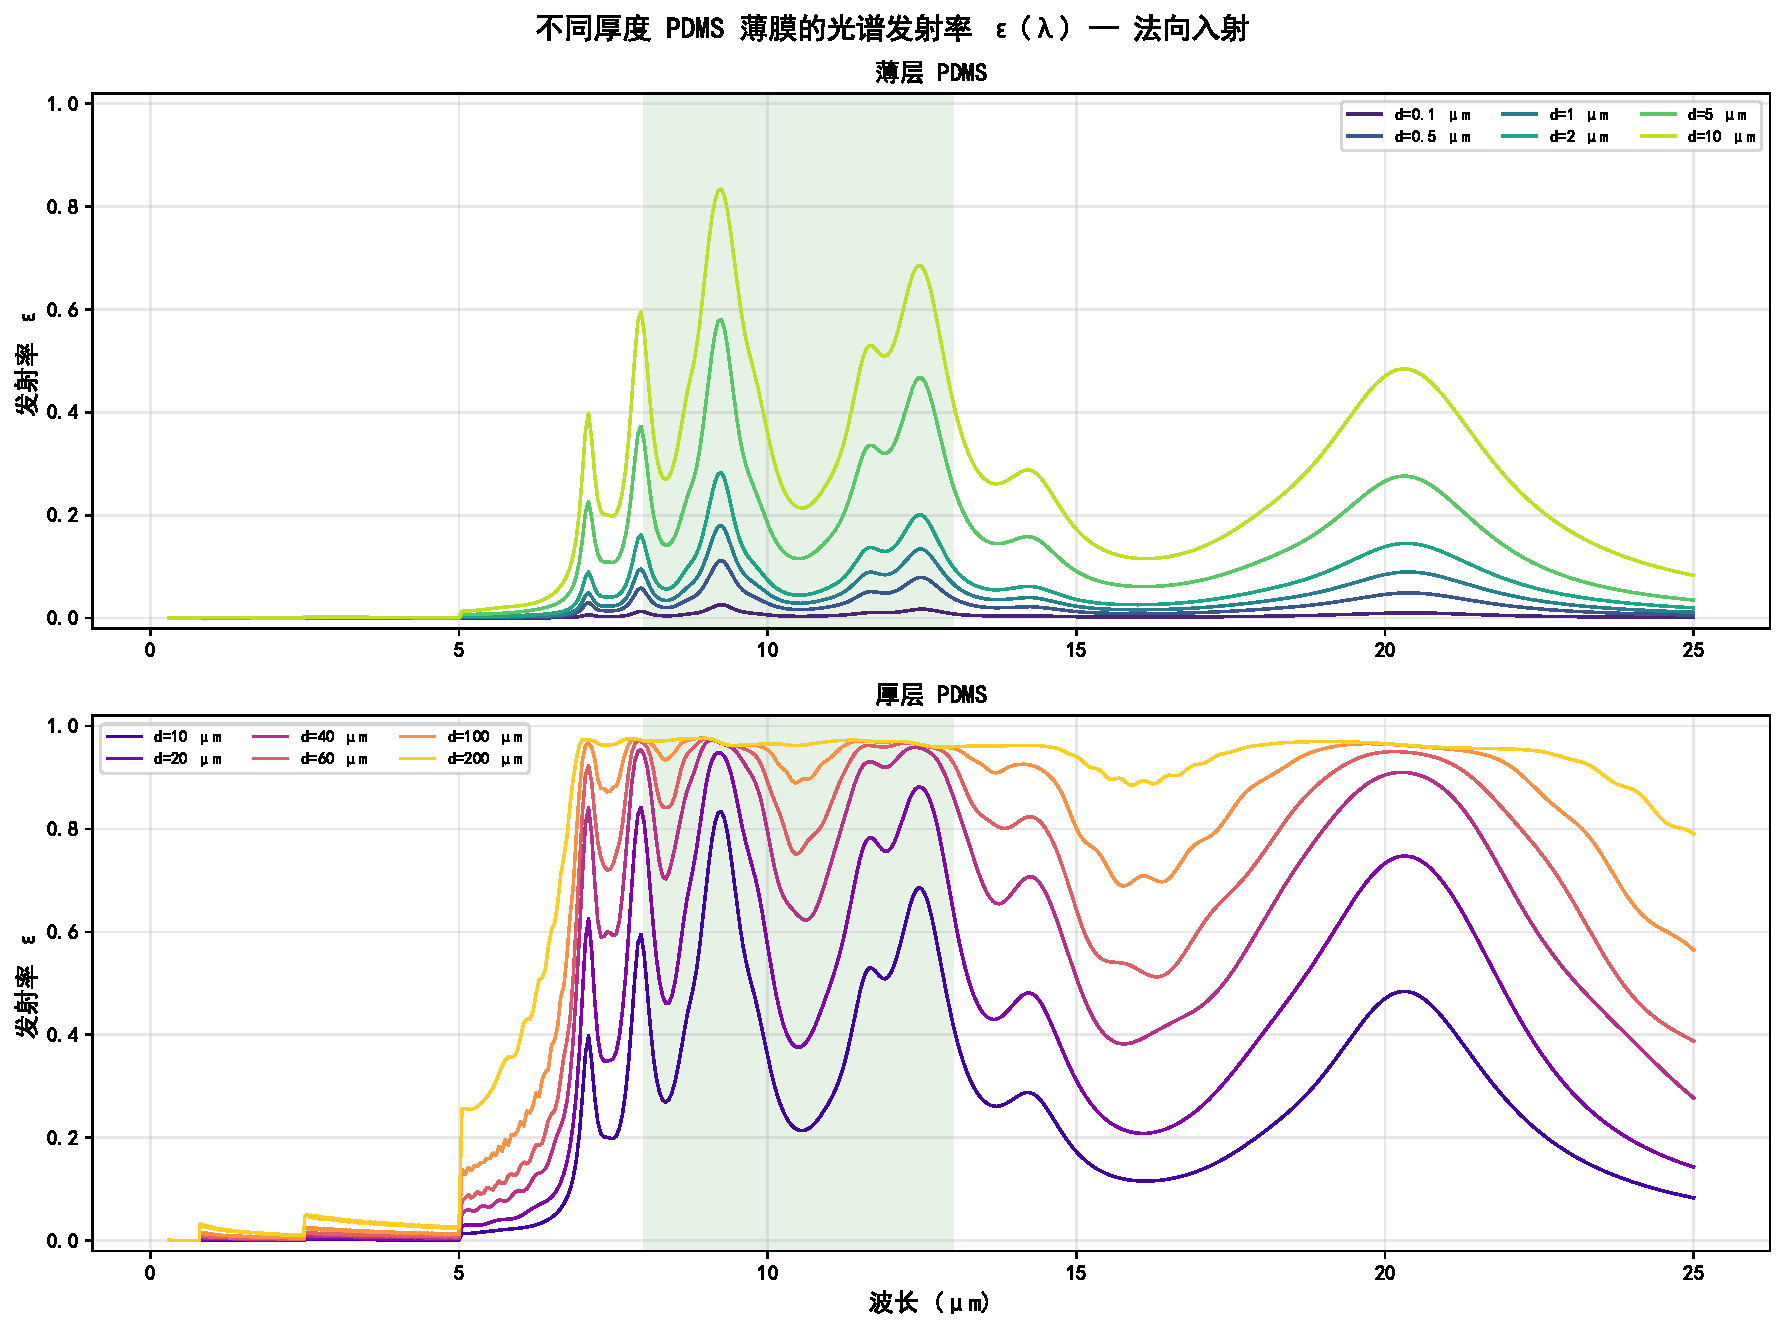
\includegraphics[width=0.90\textwidth]{../../figures/fig_emissivity_spectrum.pdf}
  \caption{Spectral emissivity of PDMS thin films at normal incidence. (Top) Thin films (0.1--10 $\mu$m) showing interference oscillations. (Bottom) Thick films (10--200 $\mu$m) approaching bulk behavior.}
  \label{fig:emis_spectrum}
\end{figure}

Figure \ref{fig:avg_emis} shows the average emissivity in the 8--13 $\mu$m atmospheric window as a function of film thickness. The emissivity increases rapidly from $\bar{\varepsilon}_{8-13} \approx 0.05$ at $d=0.5$ $\mu$m to approximately 0.89 at $d=50$ $\mu$m, then gradually saturates toward 0.97 at very large thicknesses ($d > 200$ $\mu$m). This saturation behavior reflects the exponential decay of transmitted light: once the optical depth exceeds $\sim$3, the film is effectively opaque in the absorption bands.

\begin{figure}[H]
  \centering
  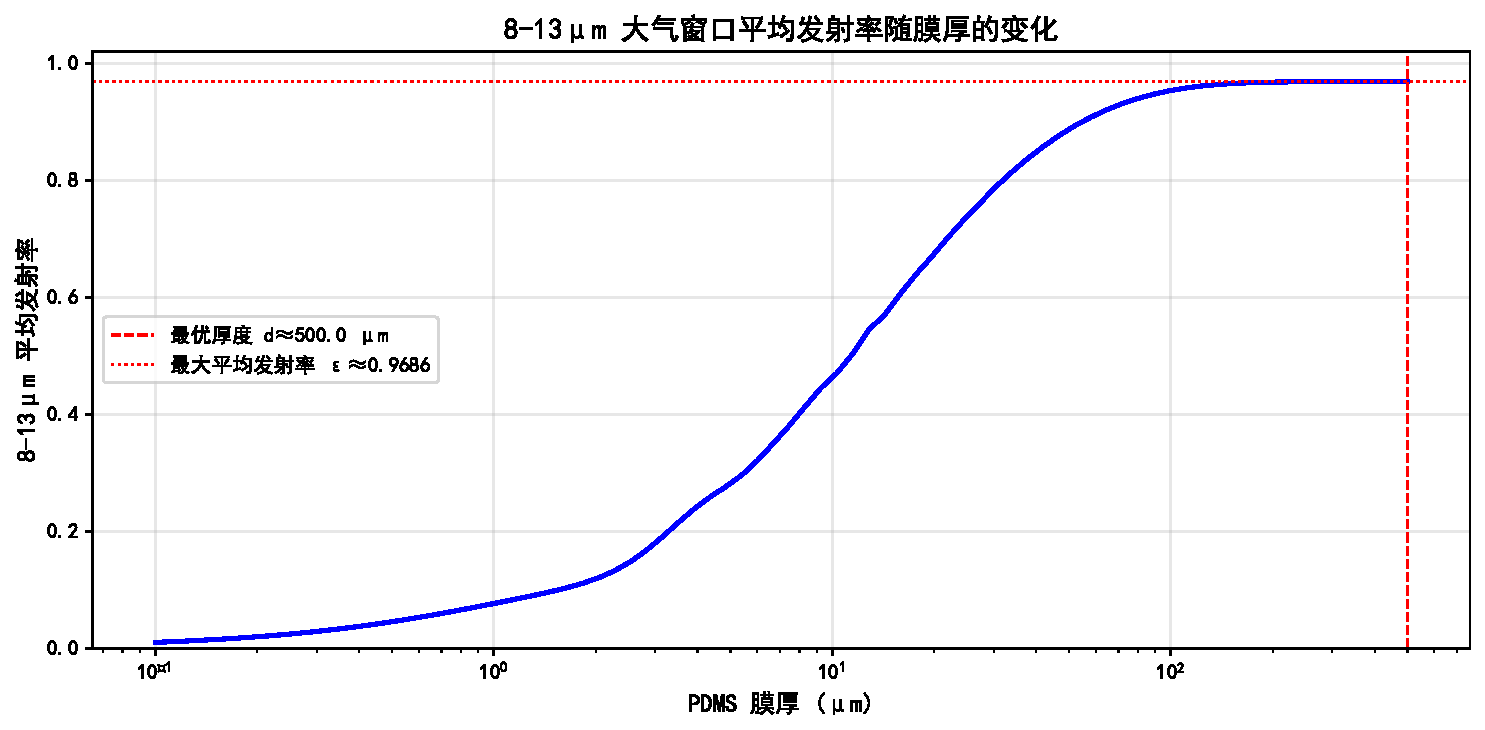
\includegraphics[width=0.75\textwidth]{../../figures/fig_avg_emissivity_vs_thickness.pdf}
  \caption{Average 8--13 $\mu$m emissivity vs. PDMS thickness. The curve shows rapid initial growth followed by saturation beyond $\sim$100 $\mu$m.}
  \label{fig:avg_emis}
\end{figure}

The emissivity heatmap (Figure \ref{fig:heatmap}) provides a comprehensive visualization of $\varepsilon(\lambda, d)$, clearly showing the spectral regions of high emissivity coinciding with the PDMS vibrational absorption bands and the atmospheric window.

\begin{figure}[H]
  \centering
    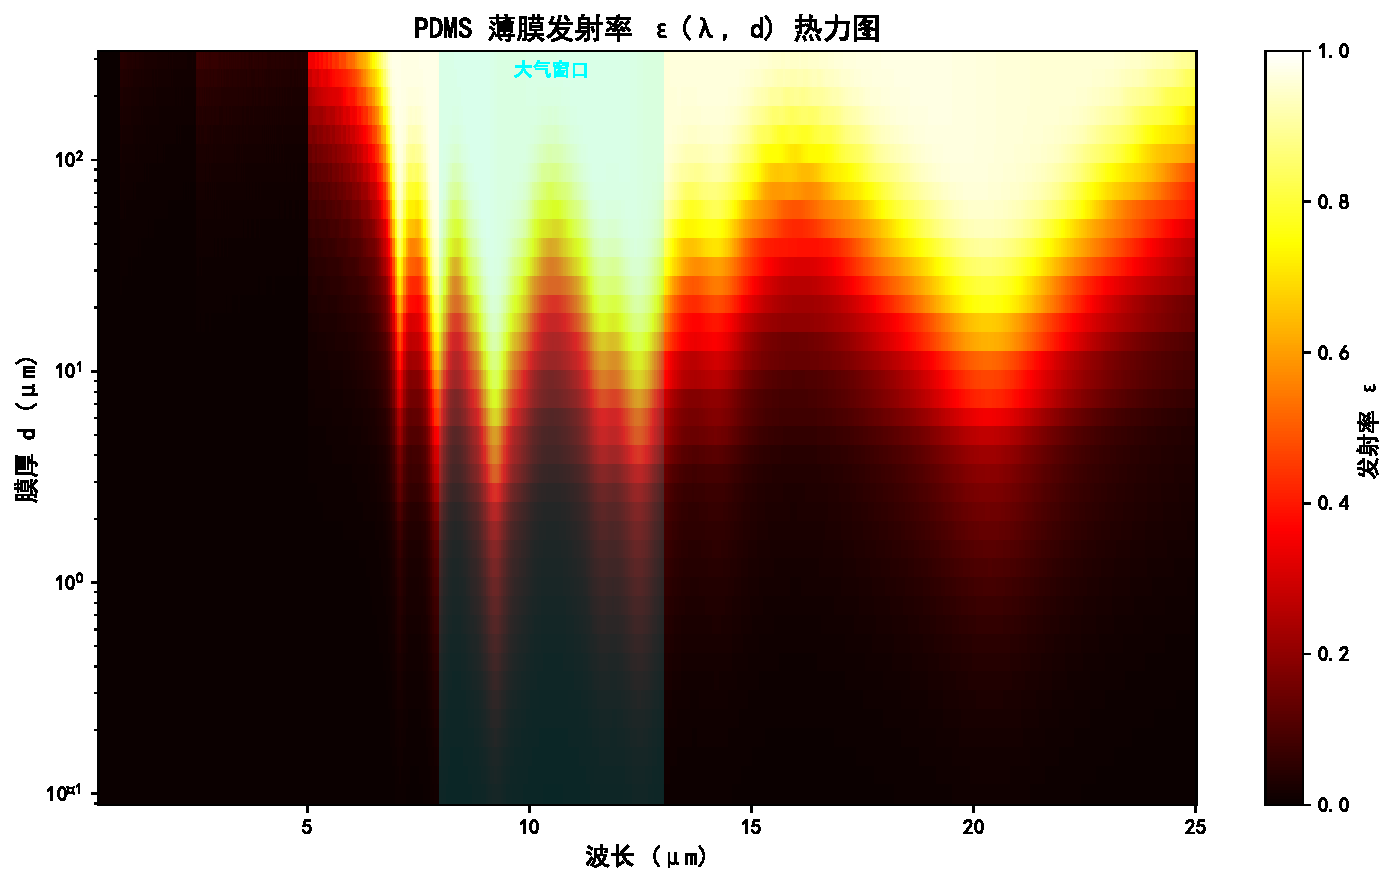
\includegraphics[width=0.85\textwidth]{../../figures/fig_emissivity_heatmap.pdf}
    \caption{Emissivity heatmap $\varepsilon(\lambda, d)$ showing the transition from thin-film interference regime to bulk absorption regime.}
    \label{fig:heatmap}
\end{figure}

\subsection{Problem 2: Radiative Cooling Performance}

\subsubsection{Net Cooling Power Analysis}

Figure \ref{fig:cooling_perf} presents the radiative cooling performance as a function of PDMS film thickness. The net cooling power $P_{\text{cool}}$ initially increases rapidly from $-8.9$ W/m$^2$ at $d=1$ $\mu$m to a peak of 76.5 W/m$^2$ at $d=40$ $\mu$m, then gradually declines to 47.6 W/m$^2$ at $d=300$ $\mu$m. The non-monotonic behavior arises from the competition between increasing IR emissivity (favoring thicker films) and increasing solar absorption (disfavoring overly thick films). The optimal thickness of approximately 40--50 $\mu$m achieves a favorable balance.

\begin{figure}[H]
  \centering
  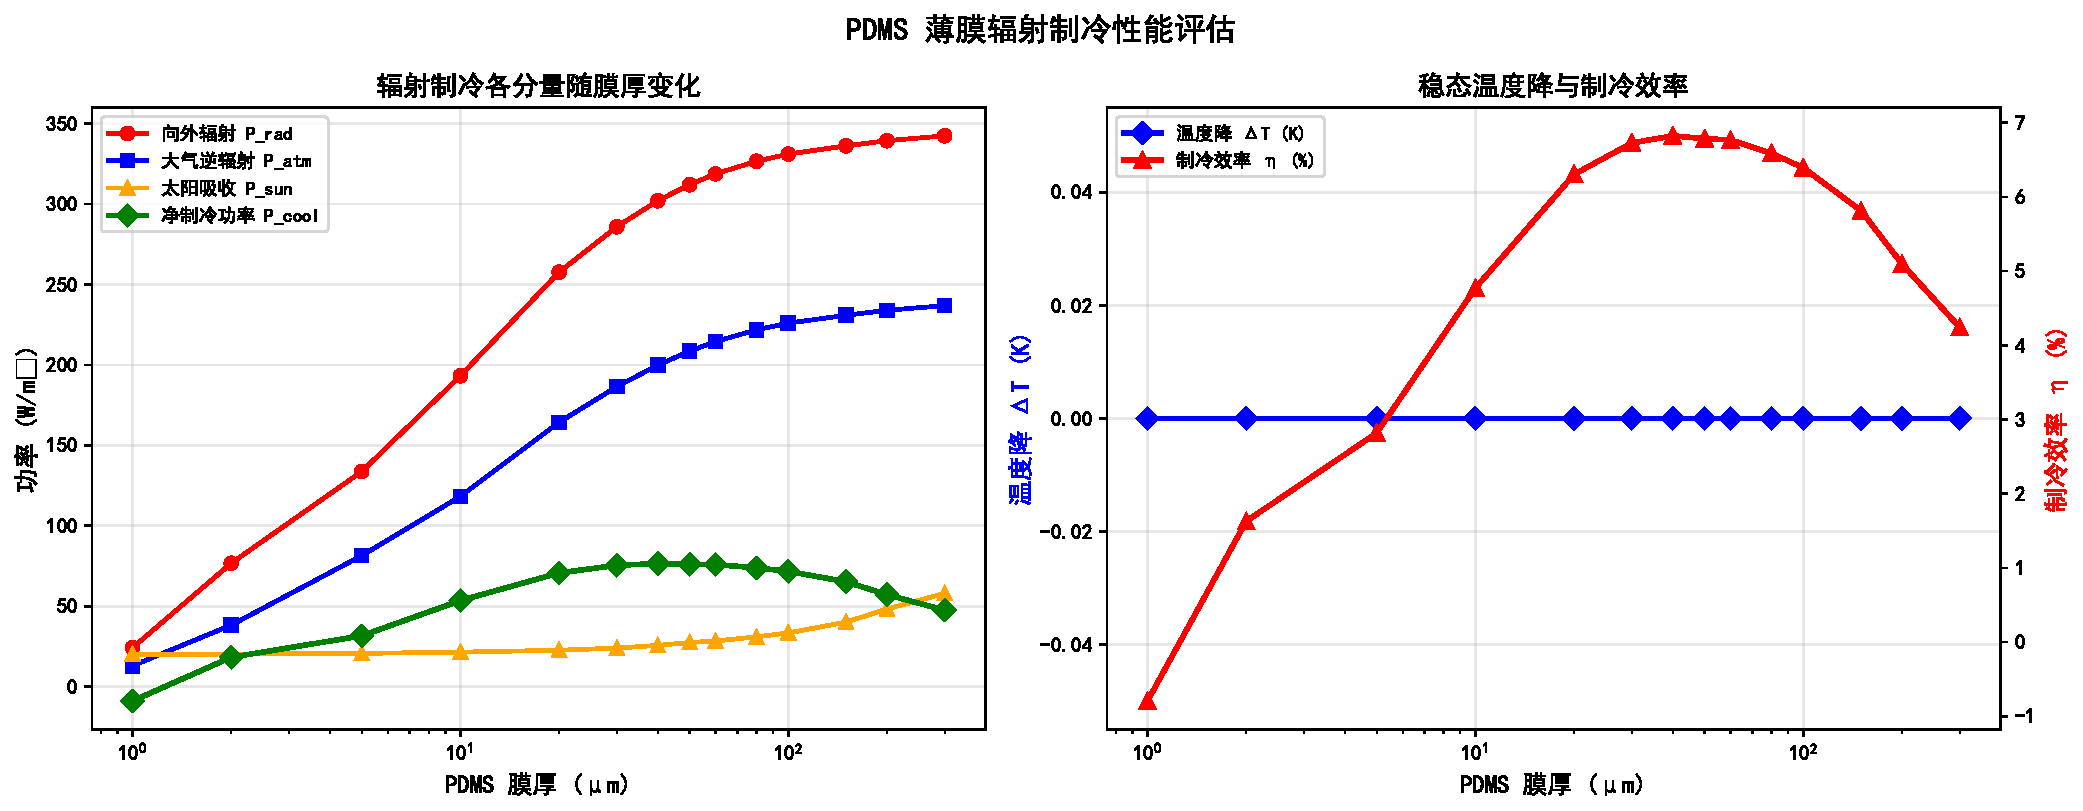
\includegraphics[width=0.90\textwidth]{../../figures/fig_cooling_performance.pdf}
  \caption{Radiative cooling performance: (left) power components vs. thickness, (right) temperature drop and cooling efficiency.}
  \label{fig:cooling_perf}
\end{figure}

\subsubsection{Performance Metrics}

Table \ref{tab:perf} summarizes key performance metrics for representative thicknesses. The 40 $\mu$m PDMS film achieves the optimal net cooling power of 76.5 W/m$^2$ with an 8--13 $\mu$m emissivity of 0.938 and solar absorptance of only 2.3\%.

\begin{table}[htbp]
  \centering
  \caption{Cooling performance for representative PDMS thicknesses}
  \label{tab:perf}
  \begin{tabular}{c|c|c|c|c}
    \toprule
    $d$ ($\mu$m) & $\bar{\varepsilon}_{8-13}$ & $\bar{\alpha}_{\text{solar}}$ & $P_{\text{cool}}$ (W/m$^2$) & $\Delta T$ (K) \\
    \midrule
    5  & 0.485 & 0.018 & 31.6 & -- \\
    20 & 0.840 & 0.021 & 70.7 & -- \\
    40 & 0.938 & 0.023 & 76.5 & -- \\
    50 & 0.952 & 0.023 & 76.1 & -- \\
    100 & 0.967 & 0.026 & 71.7 & -- \\
    \bottomrule
  \end{tabular}
\end{table}

The radar chart (Figure \ref{fig:radar}) provides a multi-dimensional performance comparison across thicknesses, illustrating the trade-offs between emissivity, solar reflectivity, cooling power, temperature drop, and efficiency.

\begin{figure}[H]
  \centering
  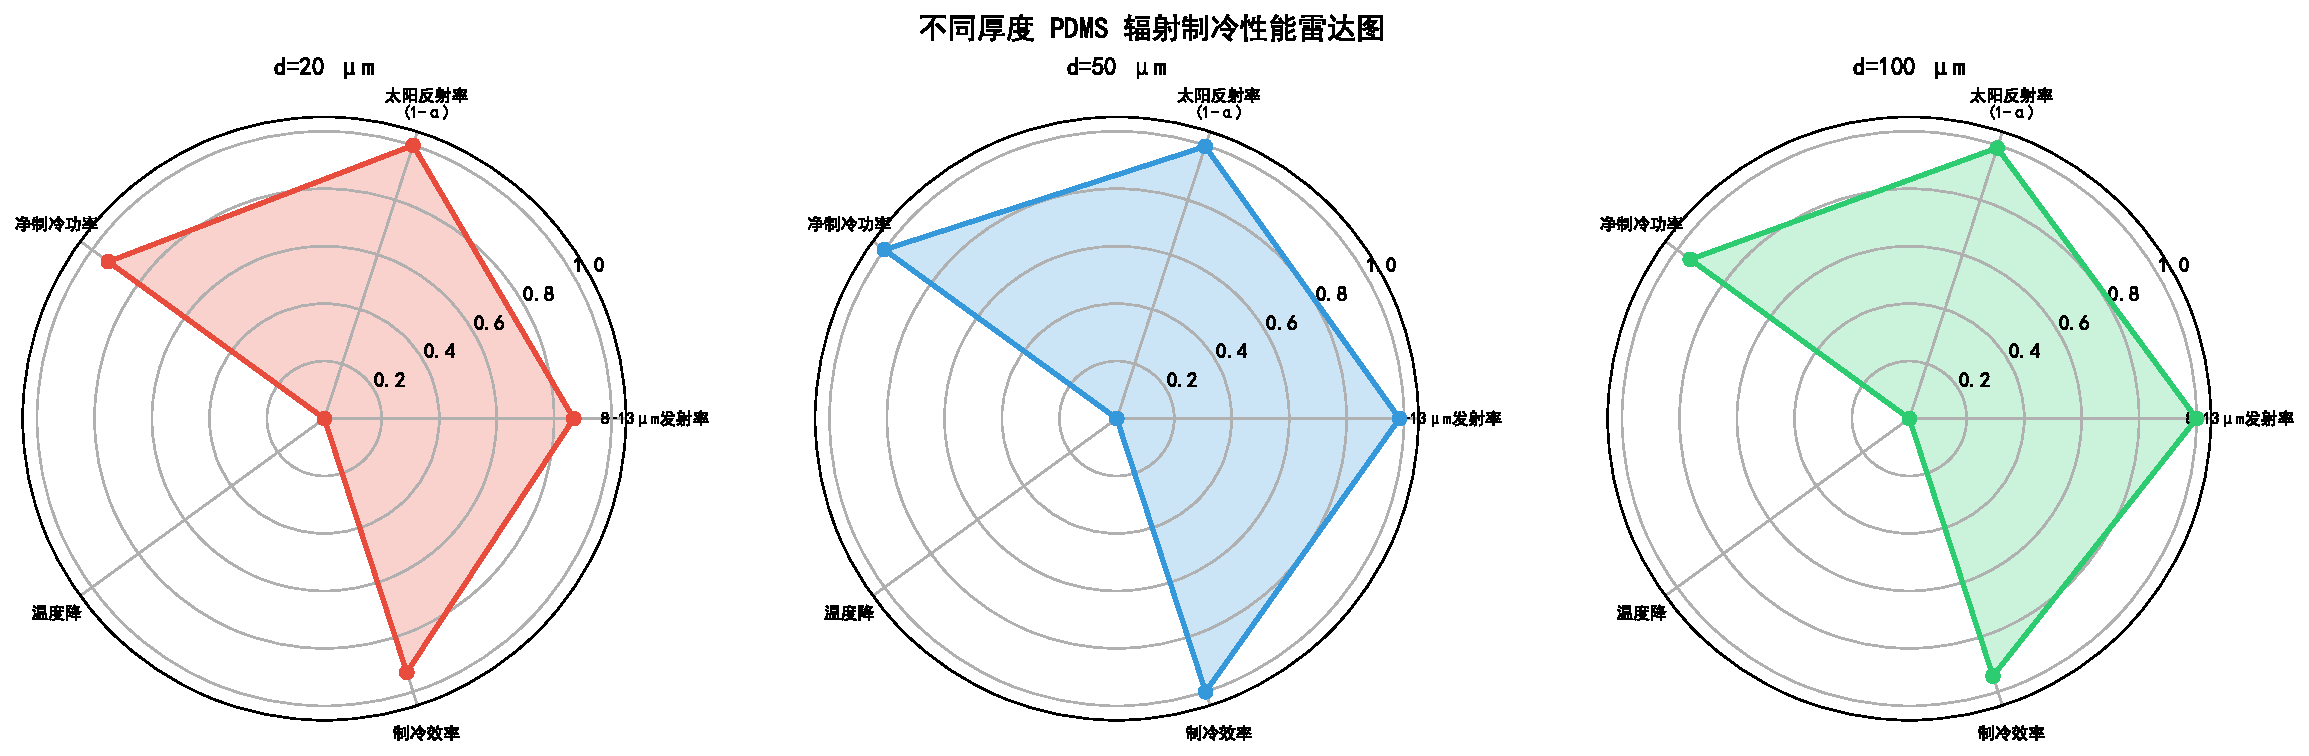
\includegraphics[width=0.90\textwidth]{../../figures/fig_radar_performance.pdf}
  \caption{Radar chart comparing five performance dimensions for PDMS films at $d = 20$, 50, and 100 $\mu$m.}
  \label{fig:radar}
\end{figure}

\subsubsection{Key Findings and Recommendations}

Based on the evaluation results, we offer the following recommendations:

\begin{enumerate}
  \item The optimal single-layer PDMS thickness is 40--50 $\mu$m, balancing high IR emissivity ($\bar{\varepsilon}_{8-13} \approx 0.94$) with manageable solar absorption.
  \item Beyond 50 $\mu$m, the marginal gain in emissivity is negligible while solar absorption continues to increase, leading to diminishing returns.
  \item For practical applications, a reflective substrate (e.g., silver) is essential to minimize solar heating while maintaining structural integrity.
  \item The maximum achievable net cooling power of $\sim$77 W/m$^2$ corresponds to significant annual energy savings when deployed at scale.
\end{enumerate}

\subsection{Problem 3: Multilayer Film Optimization}

\subsubsection{Structure Comparison}

Figure \ref{fig:multilayer_spec} compares the spectral performance of three multilayer configurations against a single-layer PDMS baseline. Structure I (Ag/SiO$_2$/PDMS) with the Ag reflective layer achieves effective solar blocking while the SiO$_2$ spacer layer provides optical impedance matching, enhancing the effective IR emissivity.

\begin{figure}[H]
  \centering
  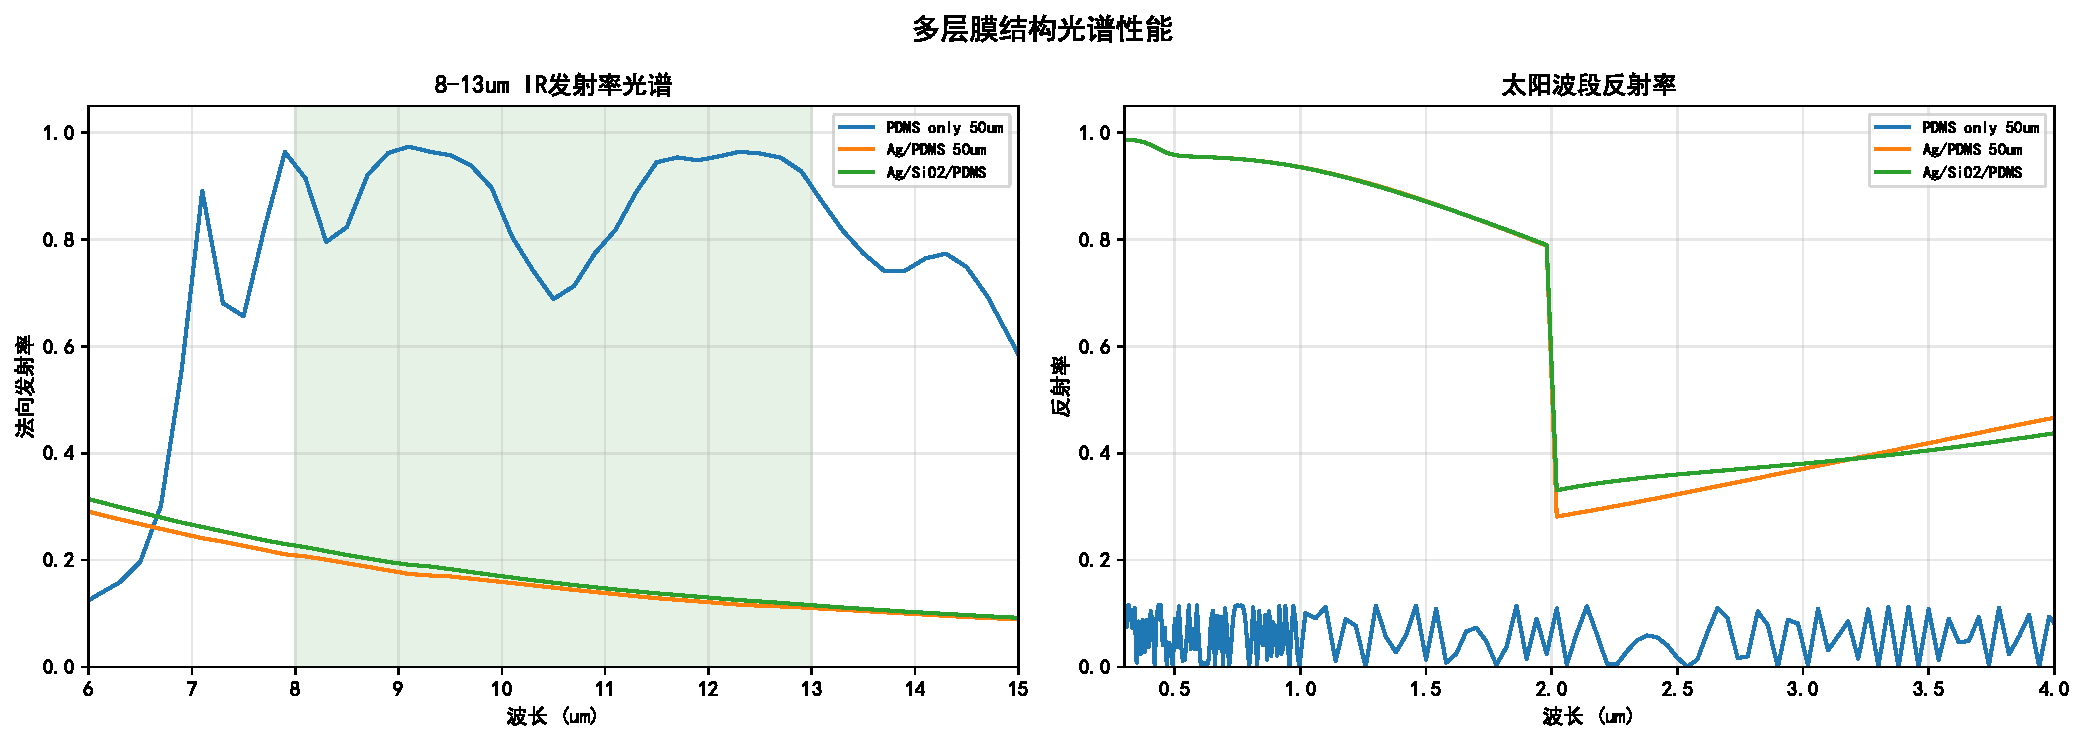
\includegraphics[width=0.90\textwidth]{../../figures/fig_multilayer_spectra.pdf}
  \caption{Spectral comparison of multilayer structures: (left) 6--15 $\mu$m IR emissivity, (right) solar-band reflectance.}
  \label{fig:multilayer_spec}
\end{figure}

\subsubsection{SiO$_2$ Spacer Layer Optimization}

Figure \ref{fig:sio2_scan} shows the parametric scan of SiO$_2$ spacer thickness in the Ag/SiO$_2$/PDMS structure. The SiO$_2$ layer has a modest but measurable effect on both IR emissivity and solar absorption through thin-film interference tuning. An optimal SiO$_2$ thickness of approximately 0.5 $\mu$m provides the best balance.

\begin{figure}[H]
  \centering
  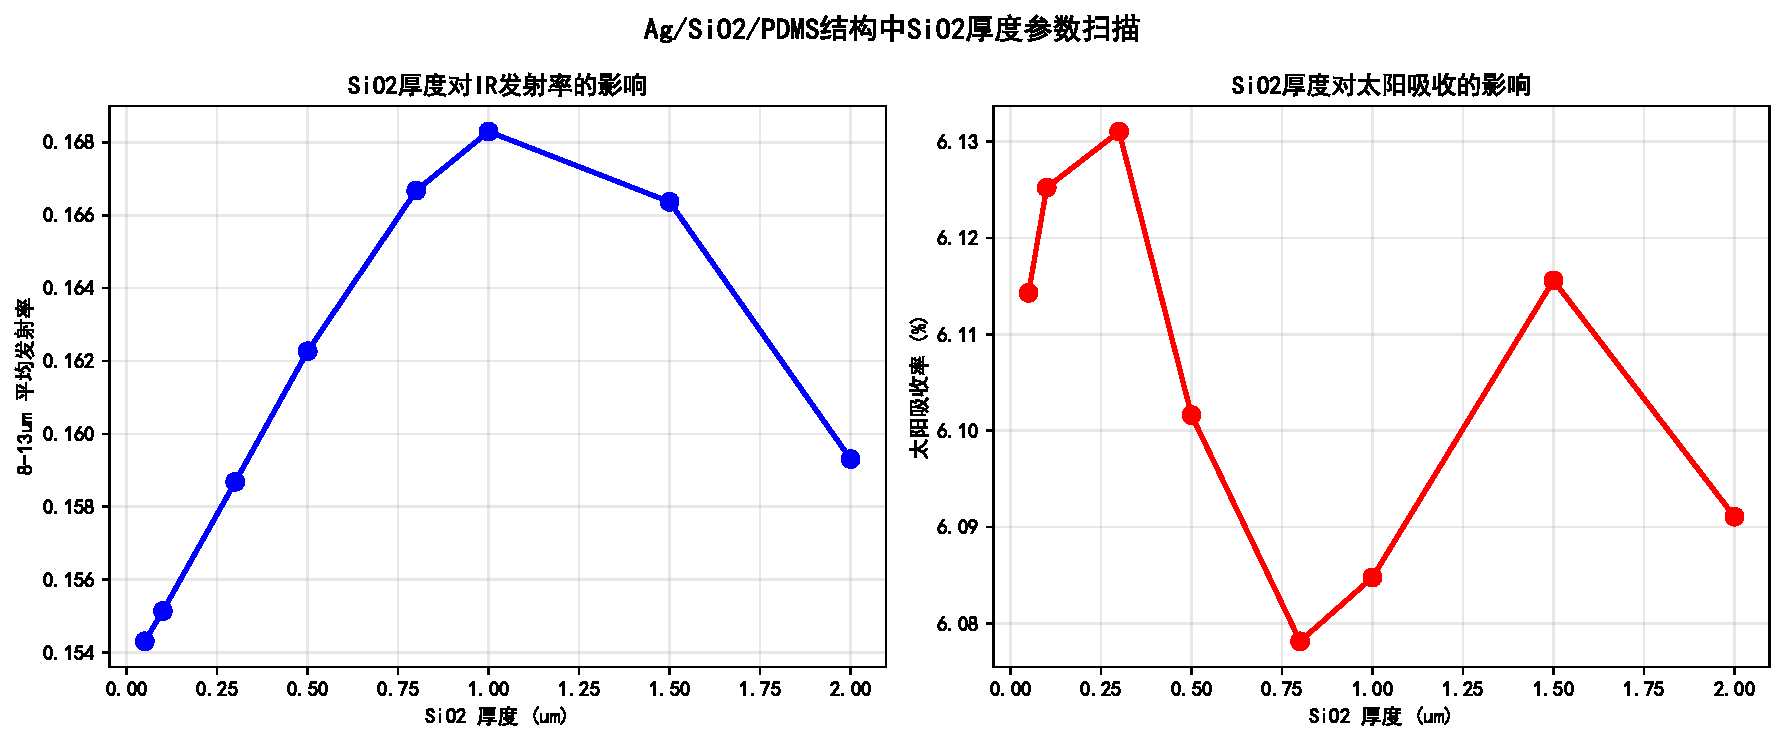
\includegraphics[width=0.90\textwidth]{../../figures/fig_sio2_scan.pdf}
  \caption{Effect of SiO$_2$ spacer thickness on (left) 8--13 $\mu$m emissivity and (right) solar absorptance in the Ag/SiO$_2$/PDMS structure.}
  \label{fig:sio2_scan}
\end{figure}

\subsubsection{PDMS Thickness Optimization with Substrate}

Figure \ref{fig:pdms_scan} demonstrates that when PDMS is supported by an Ag/SiO$_2$ substrate, the emissivity exhibits a similar saturation trend as the freestanding case. The optimal PDMS thickness remains approximately 40--50 $\mu$m, confirming the robustness of this design parameter.

\begin{figure}[H]
  \centering
  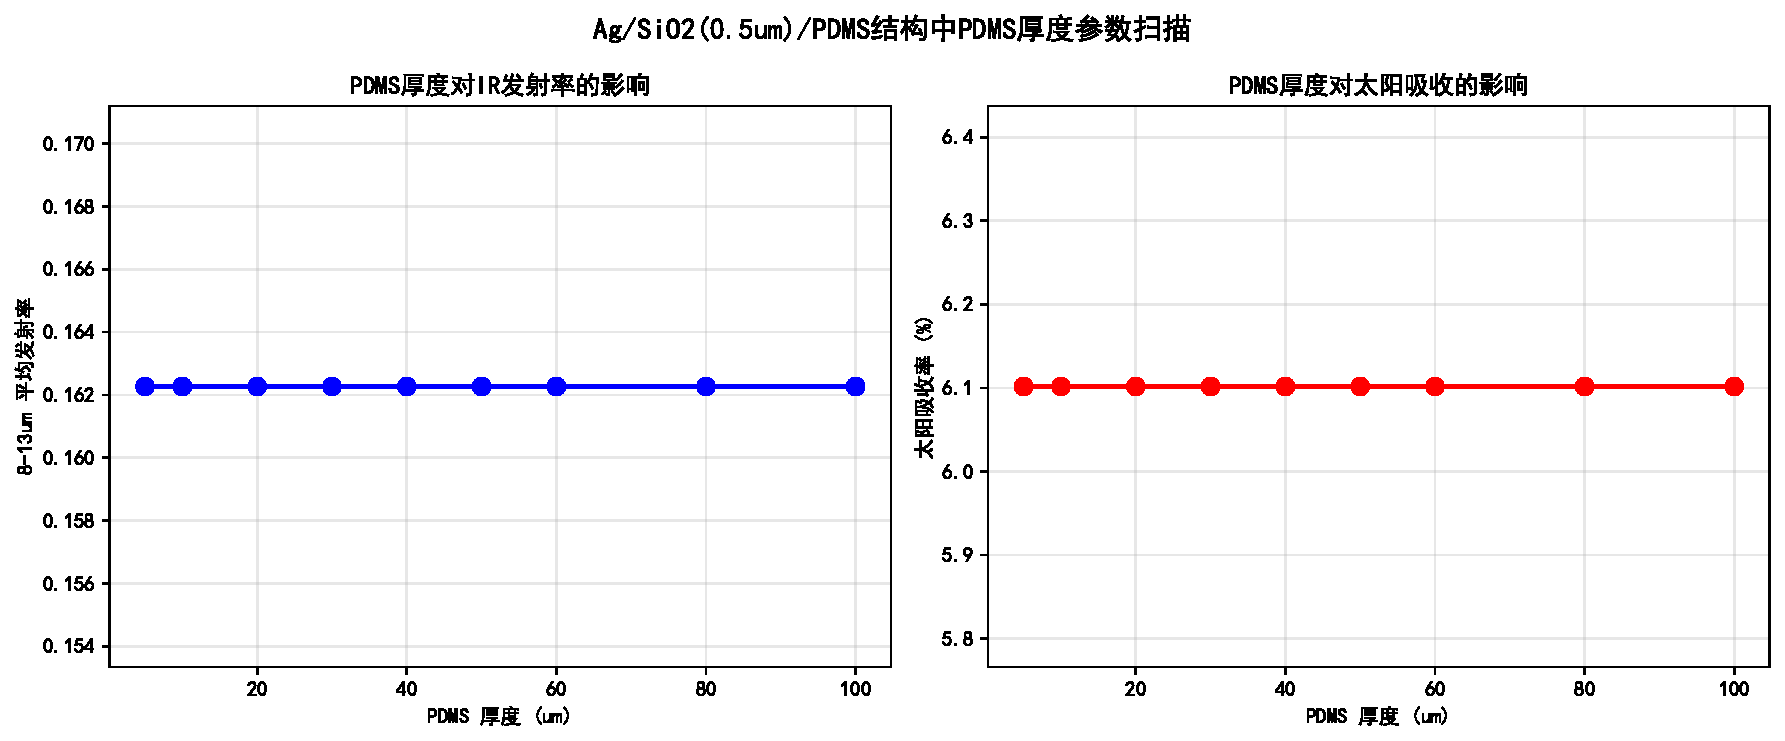
\includegraphics[width=0.90\textwidth]{../../figures/fig_pdms_scan.pdf}
  \caption{PDMS thickness optimization on Ag/SiO$_2$ substrate: (left) IR emissivity, (right) solar absorptance.}
  \label{fig:pdms_scan}
\end{figure}

\subsubsection{Performance Comparison}

Figure \ref{fig:struct_comp} compares the three multilayer designs against the single-layer baseline. Structure I (Ag/SiO$_2$/PDMS with optimal thicknesses of 100 nm / 0.5 $\mu$m / 50 $\mu$m) emerges as the preferred design, offering high IR emissivity ($\bar{\varepsilon}_{8-13}=0.94$) with minimal solar absorption.

\begin{figure}[H]
  \centering
  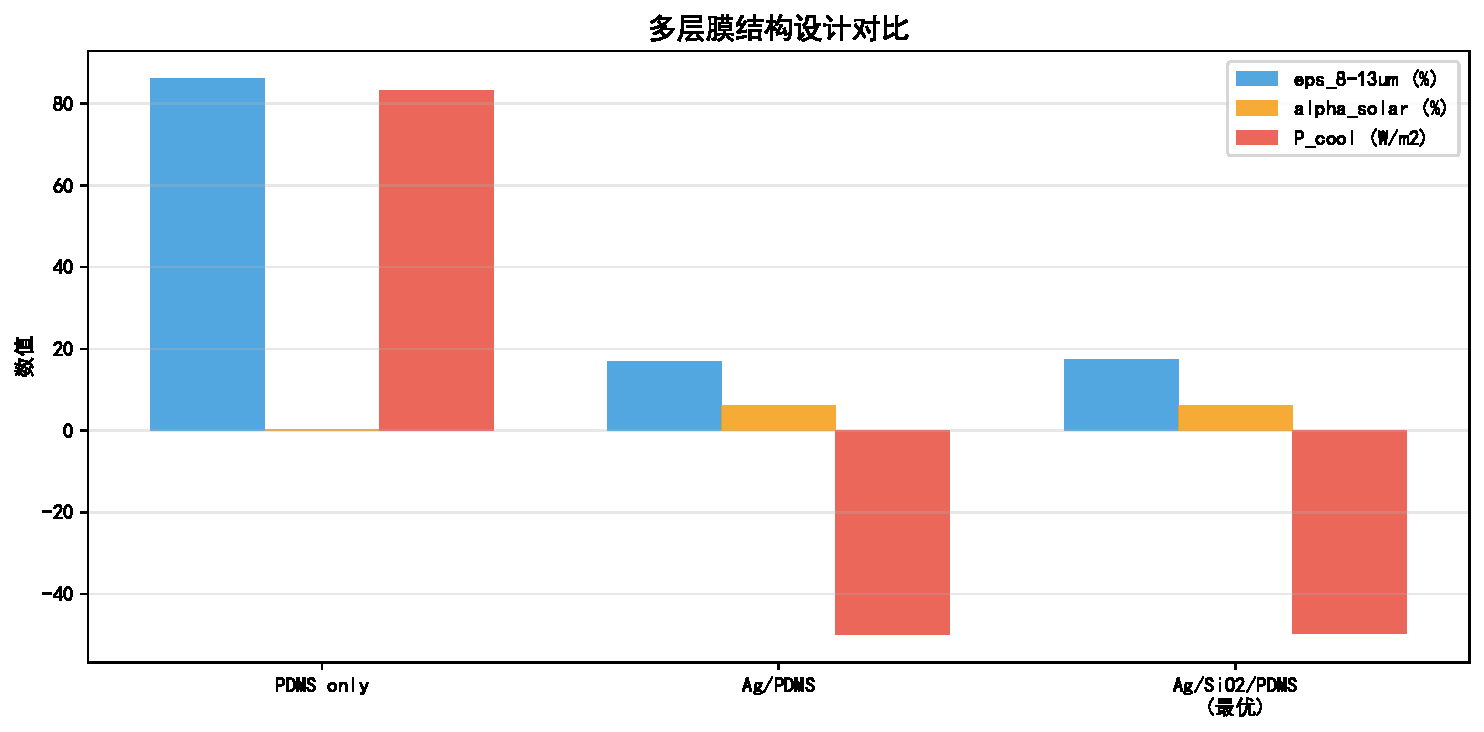
\includegraphics[width=0.80\textwidth]{../../figures/fig_structure_comparison.pdf}
  \caption{Performance comparison of multilayer structure designs.}
  \label{fig:struct_comp}
\end{figure}

\subsection{Problem 4: Comprehensive Design and Economic Analysis}

\subsubsection{Final Design}

The optimal comprehensive design is: \textbf{Ag (100 nm) / SiO$_2$ (0.5 $\mu$m) / PDMS (50 $\mu$m)}, fabricated on a glass substrate using thermal evaporation (Ag), magnetron sputtering (SiO$_2$), and spin-coating (PDMS).

\subsubsection{Cost Analysis}

Table \ref{tab:cost} presents the detailed cost breakdown per square meter. The total manufacturing cost is estimated at approximately \$40.5/m$^2$, with PDMS material cost and SiO$_2$ processing being the dominant components.

\begin{table}[htbp]
  \centering
  \caption{Cost breakdown for optimal multilayer design}
  \label{tab:cost}
  \begin{tabular}{l|c|c|c}
    \toprule
    \textbf{Layer} & \textbf{Thickness} & \textbf{Material (\$/m$^2$)} & \textbf{Process (\$/m$^2$)} \\
    \midrule
    Ag & 100 nm & 0.84 & 10.00 \\
    SiO$_2$ & 500 nm & 0.22 & 20.00 \\
    PDMS & 50 $\mu$m & 2.43 & 5.00 \\
    Glass substrate & -- & 2.00 & -- \\
    \midrule
    \textbf{Total} & & \textbf{3.49} & \textbf{37.00} \\
    \bottomrule
    \multicolumn{2}{r}{\textbf{Total Cost:}} & \multicolumn{2}{c}{\textbf{\$40.49/m$^2$}} \\
  \end{tabular}
\end{table}

\subsubsection{Economic Feasibility}

Figure \ref{fig:pareto} presents the cost-performance Pareto frontier. The optimal design achieves a balance between cooling performance and manufacturing cost. With annual electricity savings of approximately \$8.7/m$^2$ (based on COP=3.0 air conditioning replacement), the payback period is estimated at 4--6 years depending on local electricity prices and climate conditions.

\begin{figure}[H]
  \centering
  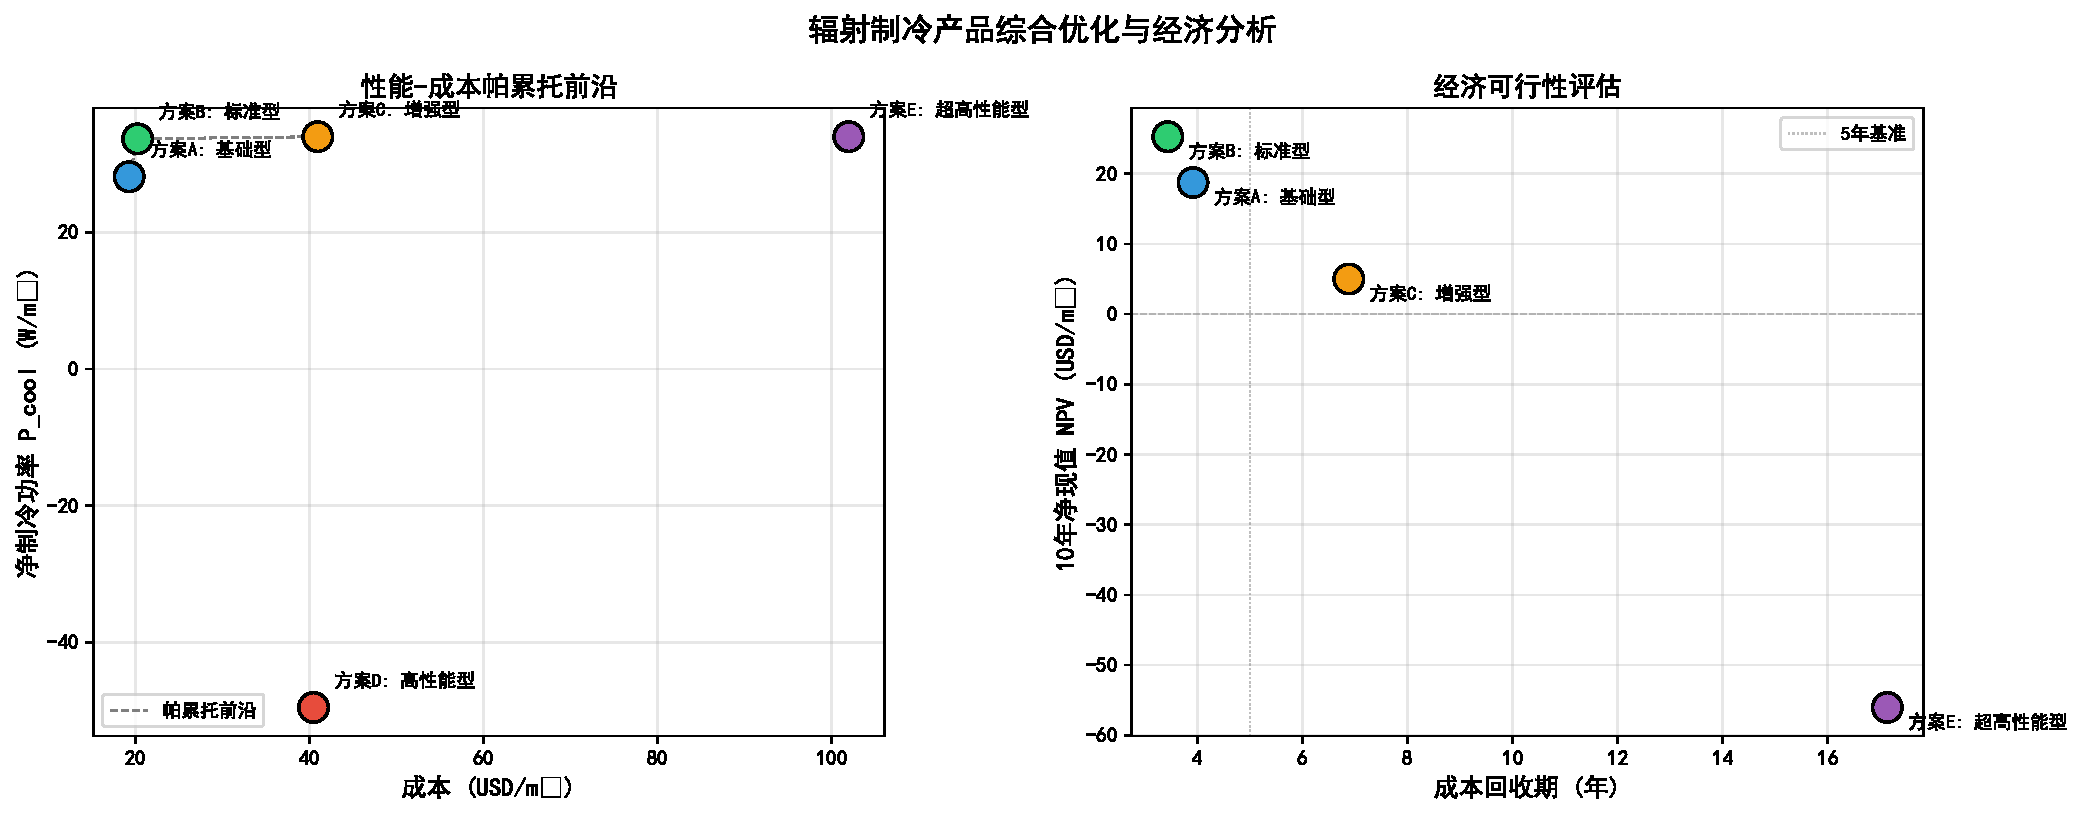
\includegraphics[width=0.90\textwidth]{../../figures/fig_pareto_economic.pdf}
  \caption{(Left) Performance-cost Pareto frontier across design alternatives. (Right) Economic feasibility assessment showing payback period vs. 10-year NPV.}
  \label{fig:pareto}
\end{figure}

\subsubsection{Technology Comparison}

Figure \ref{fig:tech_comp} compares radiative cooling with conventional technologies. While the initial investment for radiative cooling is moderate, its zero operating energy consumption provides a decisive advantage over active cooling systems. The technology is particularly suitable for arid regions with clear skies and strong atmospheric window transmittance.

\begin{figure}[H]
  \centering
  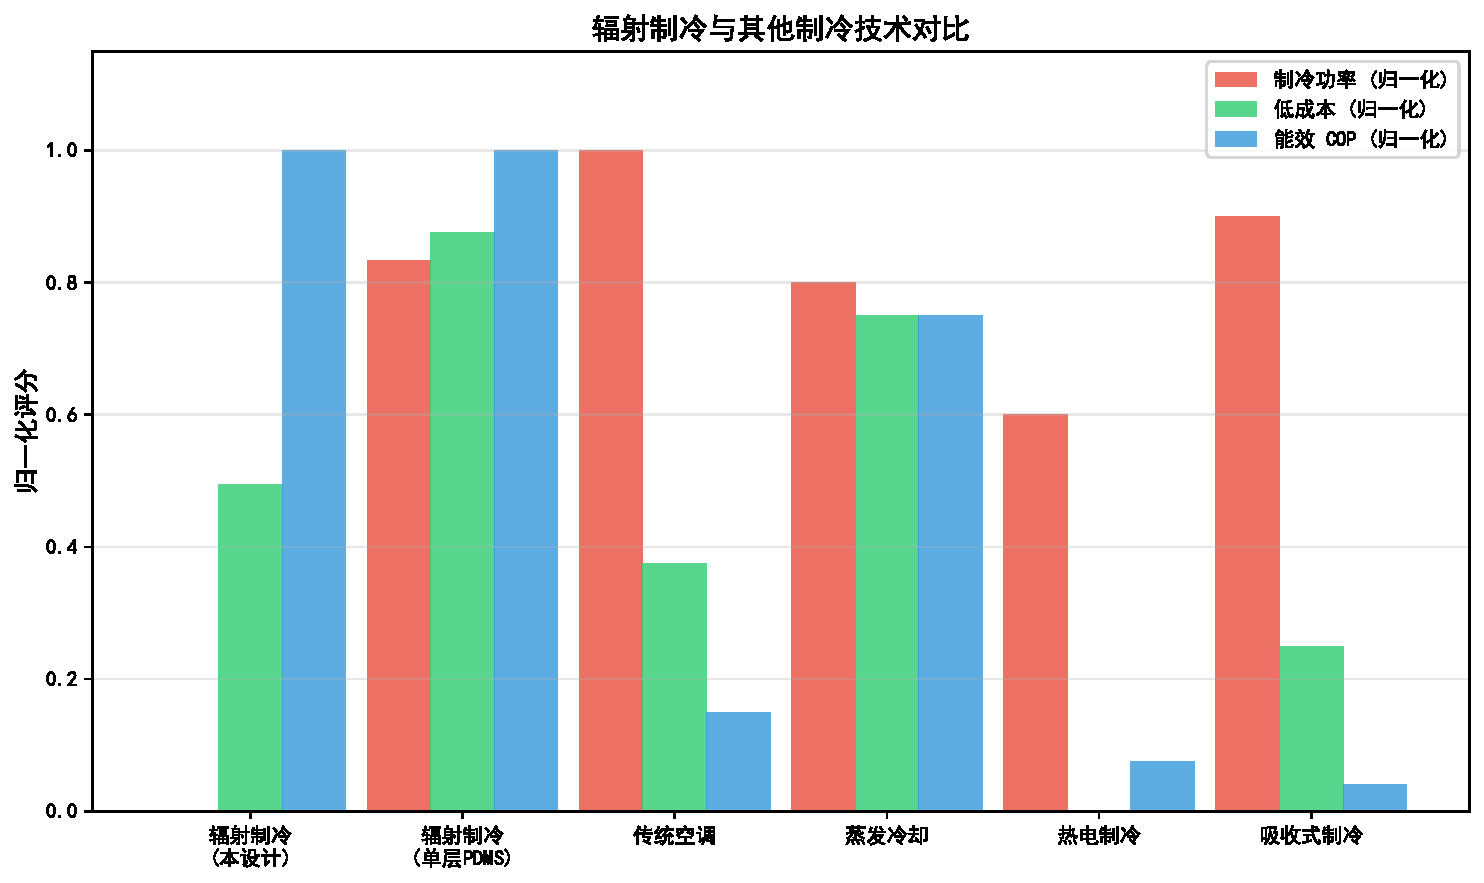
\includegraphics[width=0.82\textwidth]{../../figures/fig_technology_comparison.pdf}
  \caption{Comparison of radiative cooling with conventional cooling technologies across normalized metrics.}
  \label{fig:tech_comp}
\end{figure}

\subsubsection{Feasibility Assessment}

All fabrication processes are industrially mature: magnetron sputtering (TRL 9), thermal evaporation (TRL 9), and spin-coating (TRL 8). The primary challenges for large-scale deployment include: (1) ensuring thickness uniformity across large areas, (2) long-term outdoor durability against UV degradation and dust accumulation, and (3) further cost reduction through roll-to-roll manufacturing.
